\newpage
\pagestyle{fancy}
\lhead{\textsc{Chapitre 4. Sprint 2 --- Gestion des interventions}}
\renewcommand{\headrulewidth}{0.5pt}
\renewcommand{\footrulewidth}{0.5pt}
\chapter{Sprint 2 --- Gestion des interventions}\setlength{\headheight}{28pt}
\label{ch4}
\thispagestyle{empty}
\minitoc
\newpage

Suite à l'implémentation des fonctionnalités fondamentales du système lors du Sprint 1, ce deuxième
sprint se concentre sur la gestion des interventions préventives et correctives, la déclaration des
pannes et le calendrier des techniciens. Ce sprint constitue le noyau fonctionnel du système SAV.

Les caractéristiques élaborées au cours de ce sprint portent principalement sur :

\begin{itemize}
    \item La vérification du calendrier sur une base hebdomadaire et mensuelle ;
    \item La répartition des techniciens avec contrôle de disponibilité ;
    \item Le début et la fin des interventions par les techniciens ;
    \item Les clients peuvent déclarer des pannes avec plusieurs pièces jointes ;
    \item La gestion et la transformation des pannes en actions correctives ;
    \item L'automatisation de la vérification de la couverture contractuelle lors de la clôture.
\end{itemize}

% ─────────────────────────────────────────────────────────────────────────────
\section{Backlog du Sprint 2}

\begin{longtable}{|p{1.2cm}|p{7.5cm}|p{2.8cm}|p{1.8cm}|}
\caption{Backlog du Sprint 2 --- US-11 à US-20}
\label{tab:ch4:backlog_sprint2} \\
\hline
\textbf{ID} & \textbf{User Story} & \textbf{Acteur} & \textbf{Priorité} \\
\hline
\endfirsthead
\caption*{Backlog du Sprint 2 (suite)} \\
\hline
\textbf{ID} & \textbf{User Story} & \textbf{Acteur} & \textbf{Priorité} \\
\hline
\endhead
\hline
\endfoot
\hline
\endlastfoot
US-11 & En tant qu'administrateur, je veux affecter un technicien disponible à une intervention. & Administrateur & Élevée \\
\hline
US-12 & En tant qu'administrateur/technicien, je veux consulter le planning en vue hebdomadaire ou mensuelle. & Admin / Technicien & Élevée \\
\hline
US-13 & En tant que technicien, je veux démarrer une intervention assignée. & Technicien & Élevée \\
\hline
US-14 & En tant que technicien, je veux clôturer une intervention préventive. & Technicien & Élevée \\
\hline
US-15 & En tant que technicien, je veux clôturer une intervention curative avec vérification de la couverture contractuelle. & Technicien & Élevée \\
\hline
US-16 & En tant que client, je veux déclarer une panne sur l'un de mes équipements, avec pièces jointes. & Client & Élevée \\
\hline
US-17 & En tant qu'administrateur, je veux prendre en charge une panne et la convertir en intervention curative. & Administrateur & Élevée \\
\hline
US-18 & En tant qu'administrateur, je veux créer directement une intervention curative. & Administrateur & Élevée \\
\hline
\end{longtable}

% ─────────────────────────────────────────────────────────────────────────────
\section{Analyse}

\subsection{Diagramme de cas d'utilisation du Sprint 2}

\begin{figure}[H]
\centering
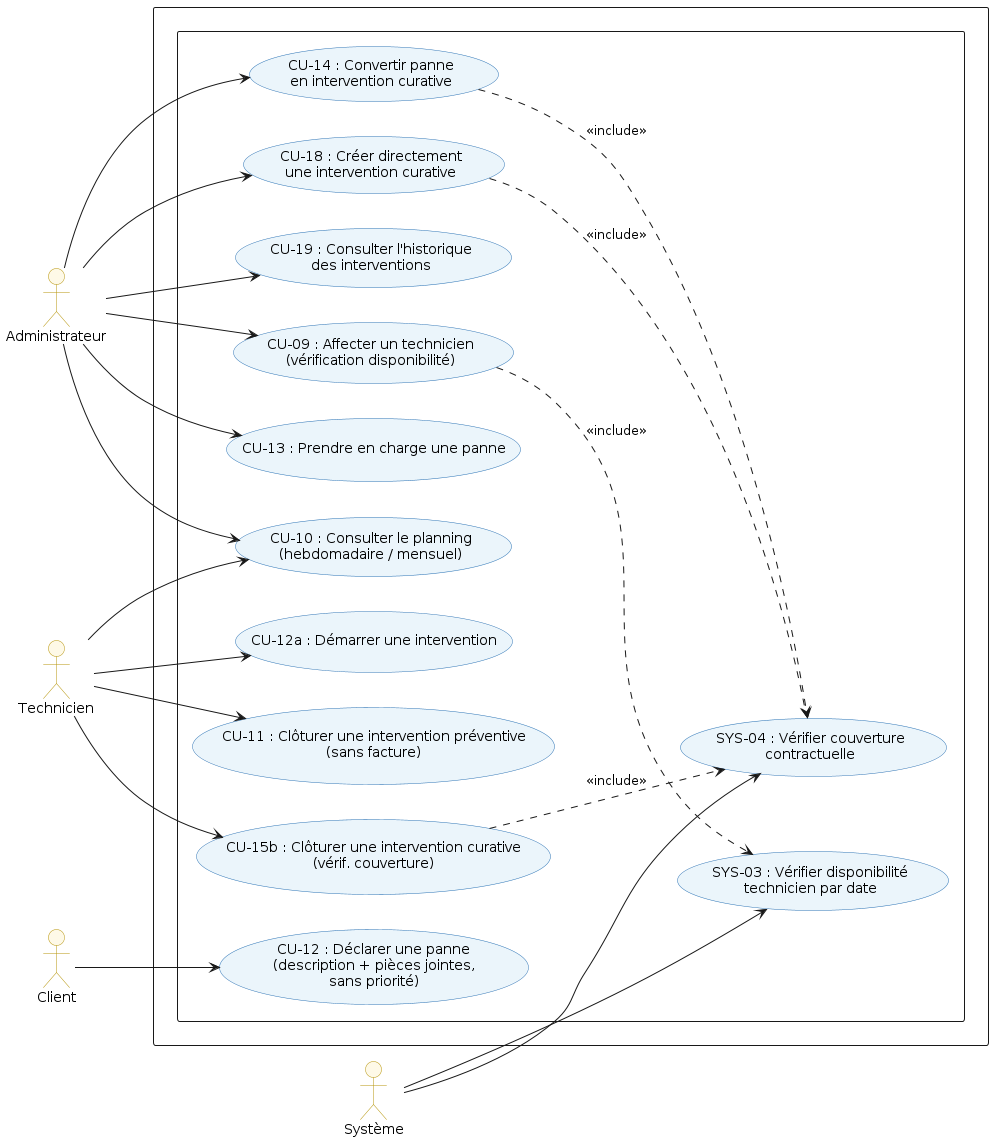
\includegraphics[width=0.70\textwidth]{Figures/Chapitre4/use_case_sprint2.png}
\caption{Diagramme de cas d'utilisation du Sprint 2}
\label{fig:ch4:usecase_sprint2}
\end{figure}

Les acteurs impliqués dans ce sprint sont :

\textbf{Administrateur} : affectation technicien, création intervention curative, prise en charge
et conversion panne, consultation planning global, historique.

\textbf{Technicien} : consultation planning personnel, démarrage et clôture d'interventions.

\textbf{Client} : déclaration de panne avec pièces jointes.

\textit{Comportements automatiques du système :} vérification de disponibilité du technicien, vérification de la couverture contractuelle.

\subsection{Description des cas d'utilisation}

\subsubsection{CU-09 : Affecter un technicien à une intervention}

\begin{table}[H]
\centering
\caption{CU-09 : Affecter un technicien à une intervention}
\label{tab:ch4:cu09}
\begin{tabular}{|p{3.5cm}|p{11cm}|}
\hline
\textbf{Champ} & \textbf{Contenu} \\
\hline
\textbf{Description}
  & Ce cas d'utilisation permet à l'administrateur d'affecter un technicien disponible
    à une intervention planifiée. \\
\hline
\textbf{Acteur principal}
  & Administrateur \\
\hline
\textbf{Préconditions}
  & L'administrateur est authentifié ; l'intervention existe ; le technicien possède
    un compte actif. \\
\hline
\textbf{Postconditions}
  & Le technicien est affecté ; le statut de l'intervention devient \texttt{PLANIFIEE} ;
    l'intervention apparaît dans le planning du technicien. \\
\hline
\end{tabular}
\end{table}

\textbf{Scénario nominal :} L'administrateur sélectionne l'intervention et le technicien à affecter ; le système vérifie l'existence, le statut et la disponibilité du technicien avant d'enregistrer l'affectation.

\textbf{Règles de gestion :}
\begin{itemize}
    \item Seuls les techniciens actifs peuvent être affectés.
    \item \textbf{Un technicien ne peut pas être affecté à deux interventions prévues à la même date.}
    \item L'affectation met automatiquement le statut de l'intervention à \texttt{PLANIFIEE}.
    \item Toute condition invalide (intervention introuvable, technicien inactif, indisponibilité à la date ou erreur technique) interrompt l'opération avec un message explicite.
\end{itemize}

\subsubsection{CU-10 : Consulter le planning}

\begin{table}[H]
\centering
\caption{CU-10 : Consulter le planning}
\label{tab:ch4:cu10}
\begin{tabular}{|p{3.5cm}|p{11cm}|}
\hline
\textbf{Champ} & \textbf{Contenu} \\
\hline
\textbf{Description}
  & Permet de consulter les interventions programmées sous forme de calendrier. \\
\hline
\textbf{Acteurs}
  & Administrateur, Technicien \\
\hline
\textbf{Préconditions}
  & Des interventions planifiées existent. \\
\hline
\textbf{Postconditions}
  & Le planning est affiché selon le rôle. \\
\hline
\end{tabular}
\end{table}

\textbf{Scénario nominal :} L'utilisateur ouvre le module Planning ; le système filtre les interventions selon le rôle et les affiche sous forme de calendrier hebdomadaire ou mensuel.

\textbf{Règles de gestion :}
\begin{itemize}
    \item Le technicien ne voit que les interventions dont il est l'affectataire.
    \item Des filtres sont disponibles pour l'administrateur (type, statut, technicien).
\end{itemize}

\subsubsection{CU-11 : Clôturer une intervention préventive}

\begin{table}[H]
\centering
\caption{CU-11 : Clôturer une intervention préventive}
\label{tab:ch4:cu11}
\begin{tabular}{|p{3.5cm}|p{11cm}|}
\hline
\textbf{Champ} & \textbf{Contenu} \\
\hline
\textbf{Description}
  & Permet au technicien de clôturer une intervention préventive réalisée. \\
\hline
\textbf{Acteur principal}
  & Technicien \\
\hline
\textbf{Préconditions}
  & Le technicien est authentifié et affecté à l'intervention ; le statut est
    \texttt{PLANIFIEE} ou \texttt{EN\_COURS}. \\
\hline
\textbf{Postconditions}
  & Le statut passe à \texttt{REALISEE} ; aucune facture n'est générée. \\
\hline
\end{tabular}
\end{table}

\textbf{Scénario nominal :} Le technicien saisit le compte rendu, les actions réalisées, le matériel utilisé et la durée ; le contrôleur vérifie l'affectation et le statut, puis met à jour l'intervention à \texttt{REALISEE}.

\textbf{Règles de gestion :}
\begin{itemize}
    \item Seul le technicien affecté peut clôturer l'intervention.
    \item \textbf{Une intervention préventive ne génère jamais de facture.}
    \item La durée est saisie en minutes.
\end{itemize}

\subsubsection{CU-12 : Déclarer une panne}

\begin{table}[H]
\centering
\caption{CU-12 : Déclarer une panne}
\label{tab:ch4:cu12}
\begin{tabular}{|p{3.5cm}|p{11cm}|}
\hline
\textbf{Champ} & \textbf{Contenu} \\
\hline
\textbf{Description}
  & Ce cas d'utilisation permet au client de signaler une panne sur l'un de ses équipements. \\
\hline
\textbf{Acteur principal}
  & Client \\
\hline
\textbf{Préconditions}
  & Le client est authentifié ; il possède au moins un équipement affecté. \\
\hline
\textbf{Postconditions}
  & La panne est enregistrée avec le statut \texttt{EN\_ATTENTE}. \\
\hline
\end{tabular}
\end{table}

\textbf{Scénario nominal :} Le client sélectionne un équipement affecté, saisit la description obligatoire et joint éventuellement des pièces jointes ; le système valide l'appartenance de l'équipement, enregistre la panne et lui attribue le statut \texttt{EN\_ATTENTE}.

\textbf{Scénarios alternatifs :}
\begin{itemize}
    \item SA1 : Description manquante $\rightarrow$ validation échoue ;
          message « Description obligatoire ».
    \item SA2 : Équipement non rattaché au client $\rightarrow$ erreur
          « Équipement introuvable ».
\end{itemize}

\textbf{Règles de gestion :}
\begin{itemize}
    \item La description est obligatoire.
    \item \textbf{Aucun champ de priorité n'est présent.}
    \item Les pièces jointes sont de type image, PDF ou audio.
    \item La panne est créée avec le statut \texttt{EN\_ATTENTE}.
\end{itemize}

\subsubsection{CU-13 : Prendre en charge une panne}

\begin{table}[H]
\centering
\caption{CU-13 : Prendre en charge une panne}
\label{tab:ch4:cu13}
\begin{tabular}{|p{3.5cm}|p{11cm}|}
\hline
\textbf{Champ} & \textbf{Contenu} \\
\hline
\textbf{Description}
  & Permet à l'administrateur de prendre en charge une panne déclarée. \\
\hline
\textbf{Acteur principal}
  & Administrateur \\
\hline
\textbf{Préconditions}
  & Une panne a été déclarée avec le statut \texttt{EN\_ATTENTE}. \\
\hline
\textbf{Postconditions}
  & Le statut de la panne passe à \texttt{PRISE\_EN\_CHARGE}. \\
\hline
\end{tabular}
\end{table}

\textbf{Scénario nominal :} L'administrateur sélectionne une panne \texttt{EN\_ATTENTE} et déclenche la prise en charge ; le statut est mis à jour à \texttt{PRISE\_EN\_CHARGE}.

\subsubsection{CU-14 : Convertir une panne en intervention curative}

\begin{table}[H]
\centering
\caption{CU-14 : Convertir une panne en intervention curative}
\label{tab:ch4:cu14}
\begin{tabular}{|p{3.5cm}|p{11cm}|}
\hline
\textbf{Champ} & \textbf{Contenu} \\
\hline
\textbf{Description}
  & Permet à l'administrateur de convertir une panne en intervention curative afin
    d'organiser le traitement technique. \\
\hline
\textbf{Acteur principal}
  & Administrateur \\
\hline
\textbf{Préconditions}
  & Une panne est en statut \texttt{EN\_ATTENTE} ou \texttt{PRISE\_EN\_CHARGE}. \\
\hline
\textbf{Postconditions}
  & Une intervention curative est créée ; la panne passe au statut \texttt{CONVERTIE}. \\
\hline
\end{tabular}
\end{table}

\textbf{Scénario nominal :} L'administrateur sélectionne la panne à convertir, saisit la date prévue et affecte optionnellement un technicien disponible ; le système crée l'intervention curative liée à la panne, vérifie automatiquement la couverture contractuelle, renseigne \texttt{couvertureContrat} et fait passer la panne au statut \texttt{CONVERTIE}.

\textbf{Règles de gestion :}
\begin{itemize}
    \item \textbf{Aucun champ de priorité n'est associé à l'intervention curative créée.}
    \item La couverture contractuelle est vérifiée automatiquement par le Système : si un contrat actif couvre l'installation \texttt{ClientEquipement} à la date de l'intervention, \texttt{couvertureContrat} = true ; sinon false.
    \item Si un technicien est affecté, la disponibilité est vérifiée.
\end{itemize}

% ─────────────────────────────────────────────────────────────────────────────
\section{Conception}

\subsection{Diagramme de classes du Sprint 2}

\begin{figure}[H]
\centering
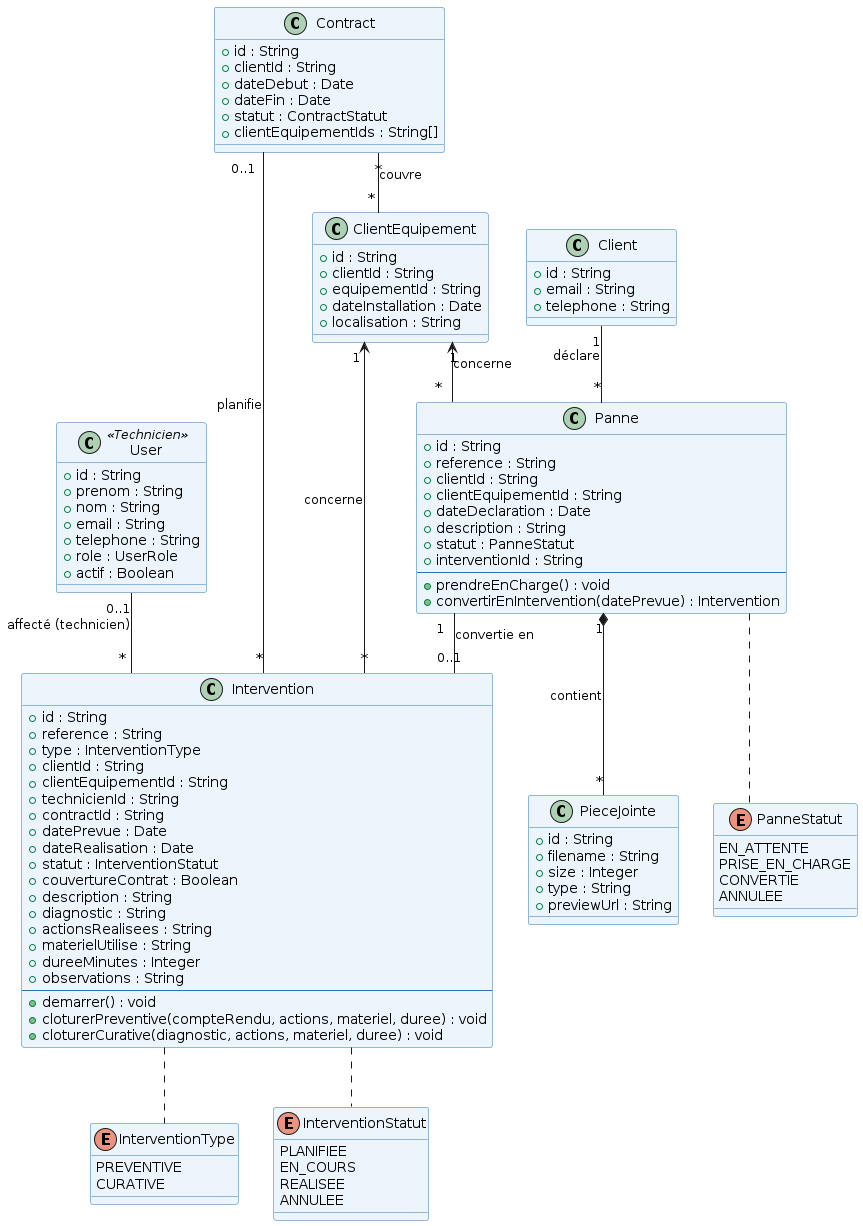
\includegraphics[width=0.70\textwidth]{Figures/Chapitre4/class_diagram_sprint2.png}
\caption{Diagramme de classes du Sprint 2}
\label{fig:ch4:class_sprint2}
\end{figure}

Les entités impliquées dans ce sprint sont : \texttt{Intervention}, \texttt{Panne},
\texttt{PieceJointe}, \texttt{Contract}, \texttt{ClientEquipement}, \texttt{User} (technicien).

\subsection{Diagrammes de séquence}

La génération du planning préventif est déclenchée lors de la création du contrat, comme présenté dans le Sprint 1.

\subsubsection{Diagramme de séquence : Clôture intervention curative et vérification couverture}

\begin{figure}[H]
\centering
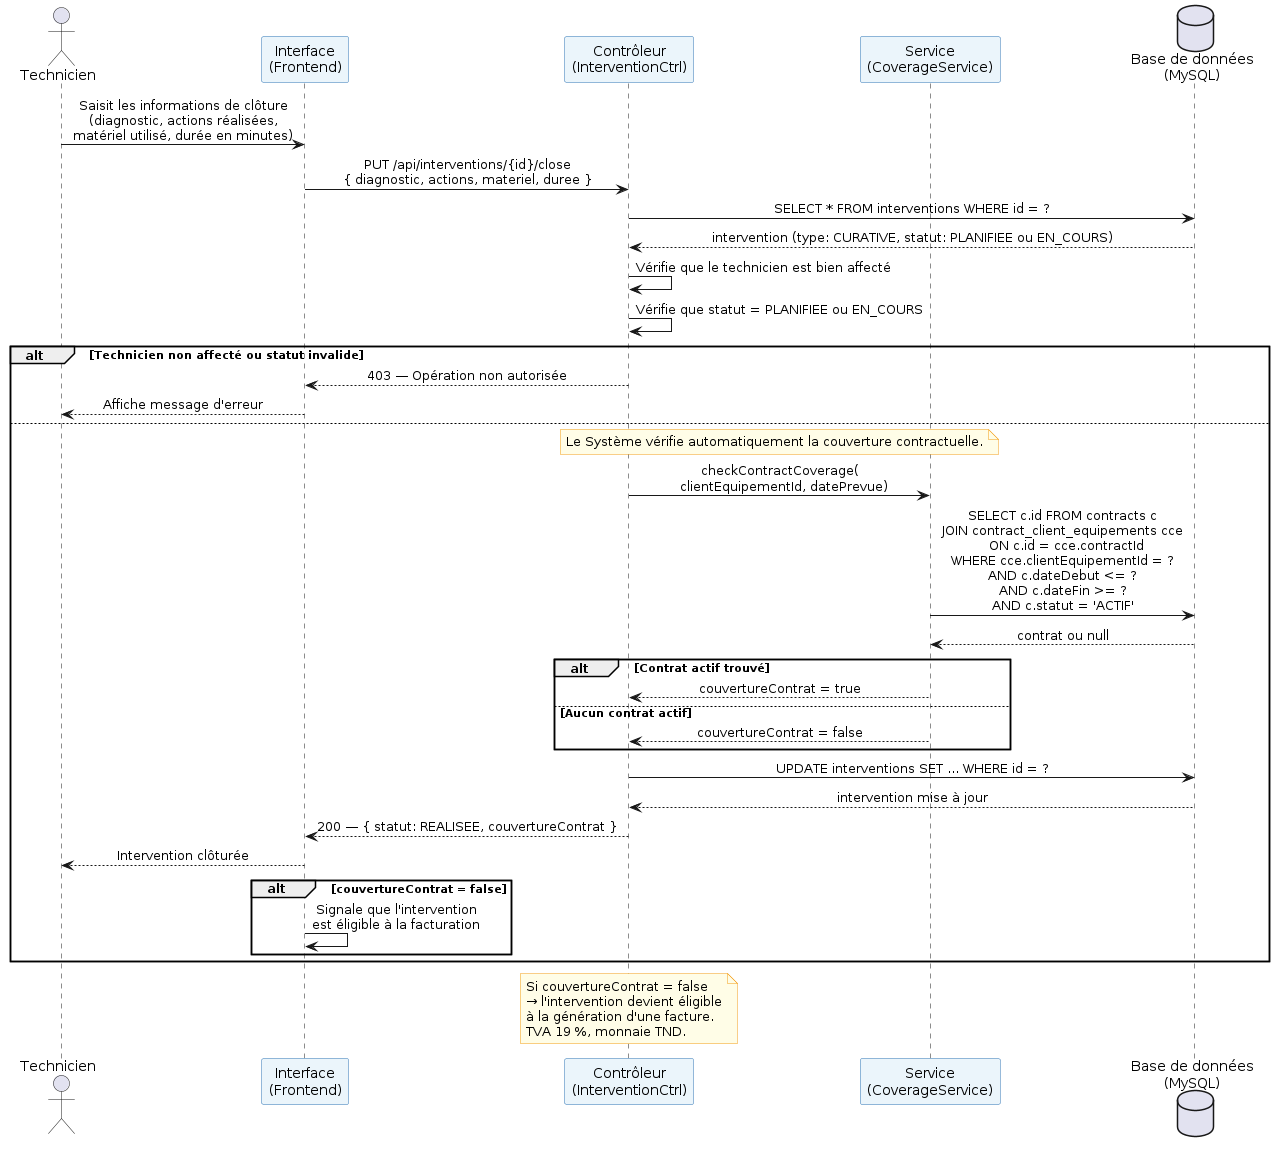
\includegraphics[width=0.70\textwidth]{Figures/Chapitre4/seq_cloturercurative_sprint2.png}
\caption{Diagramme de séquence : Clôture intervention curative et vérification couverture}
\label{fig:ch4:seq_cloture_curative}
\end{figure}

% ─────────────────────────────────────────────────────────────────────────────
\section{Réalisation}

\begin{figure}[H]
    \centering
    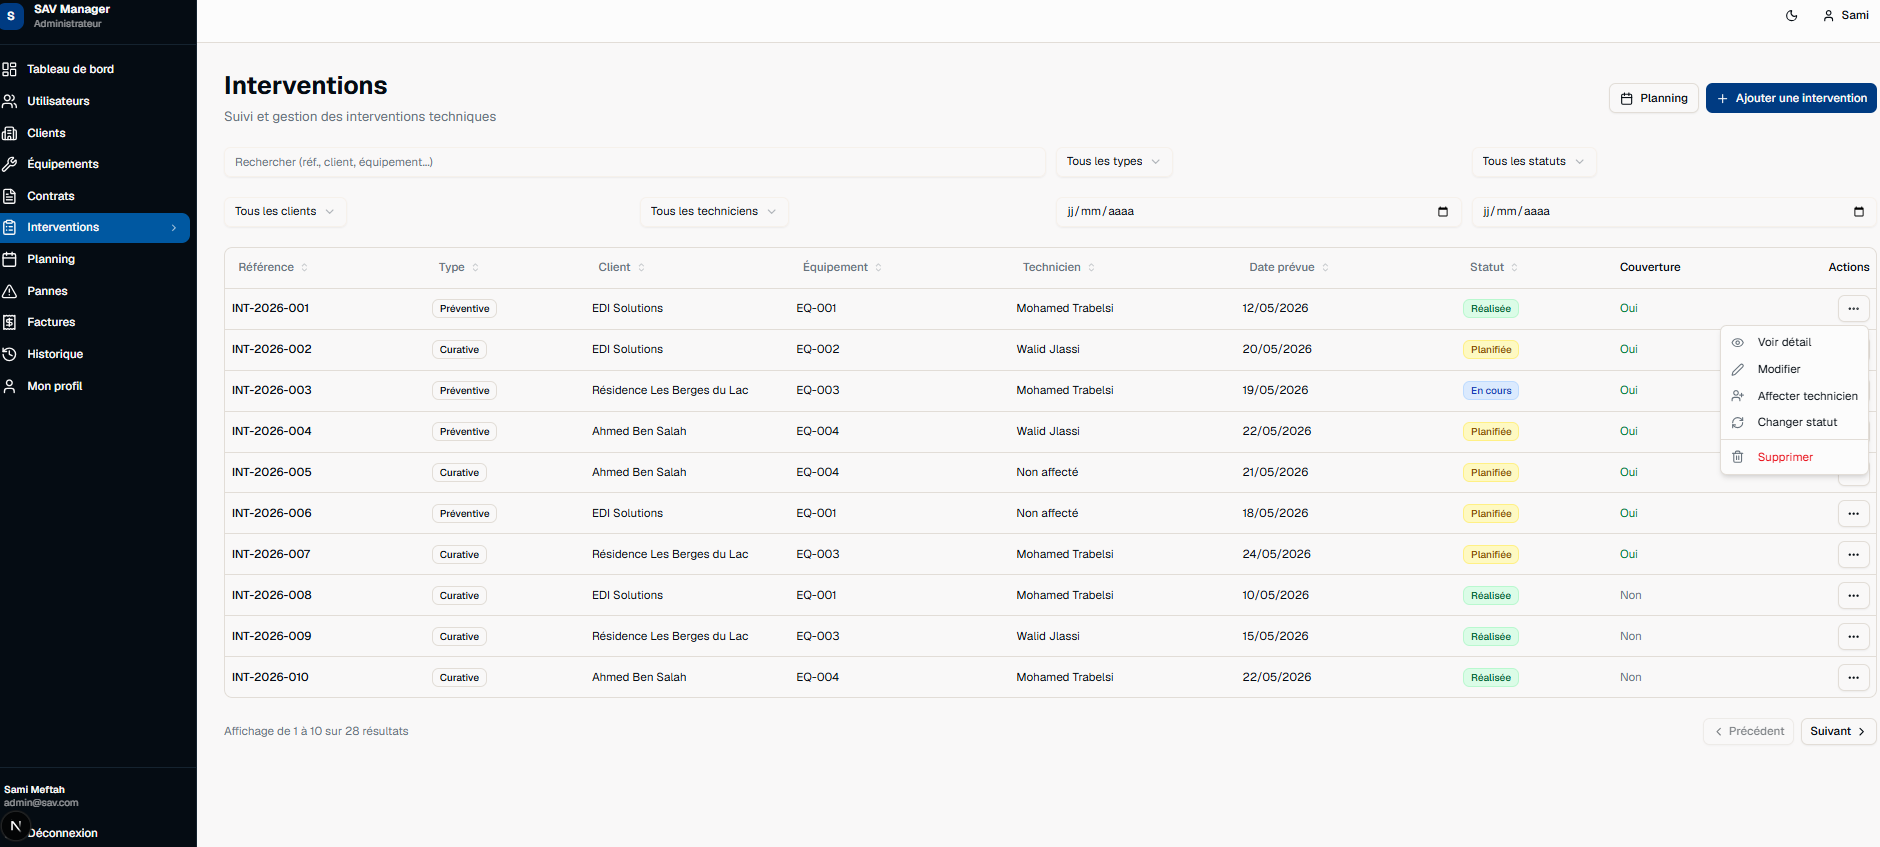
\includegraphics[width=0.74\textwidth]{Figures/Chapitre4/gestintervention.png}
    \caption{Capture d'écran : gestion des interventions}
    \label{fig:ch4:realisation_sprint2_interventions}
\end{figure}

\begin{figure}[H]
    \centering
    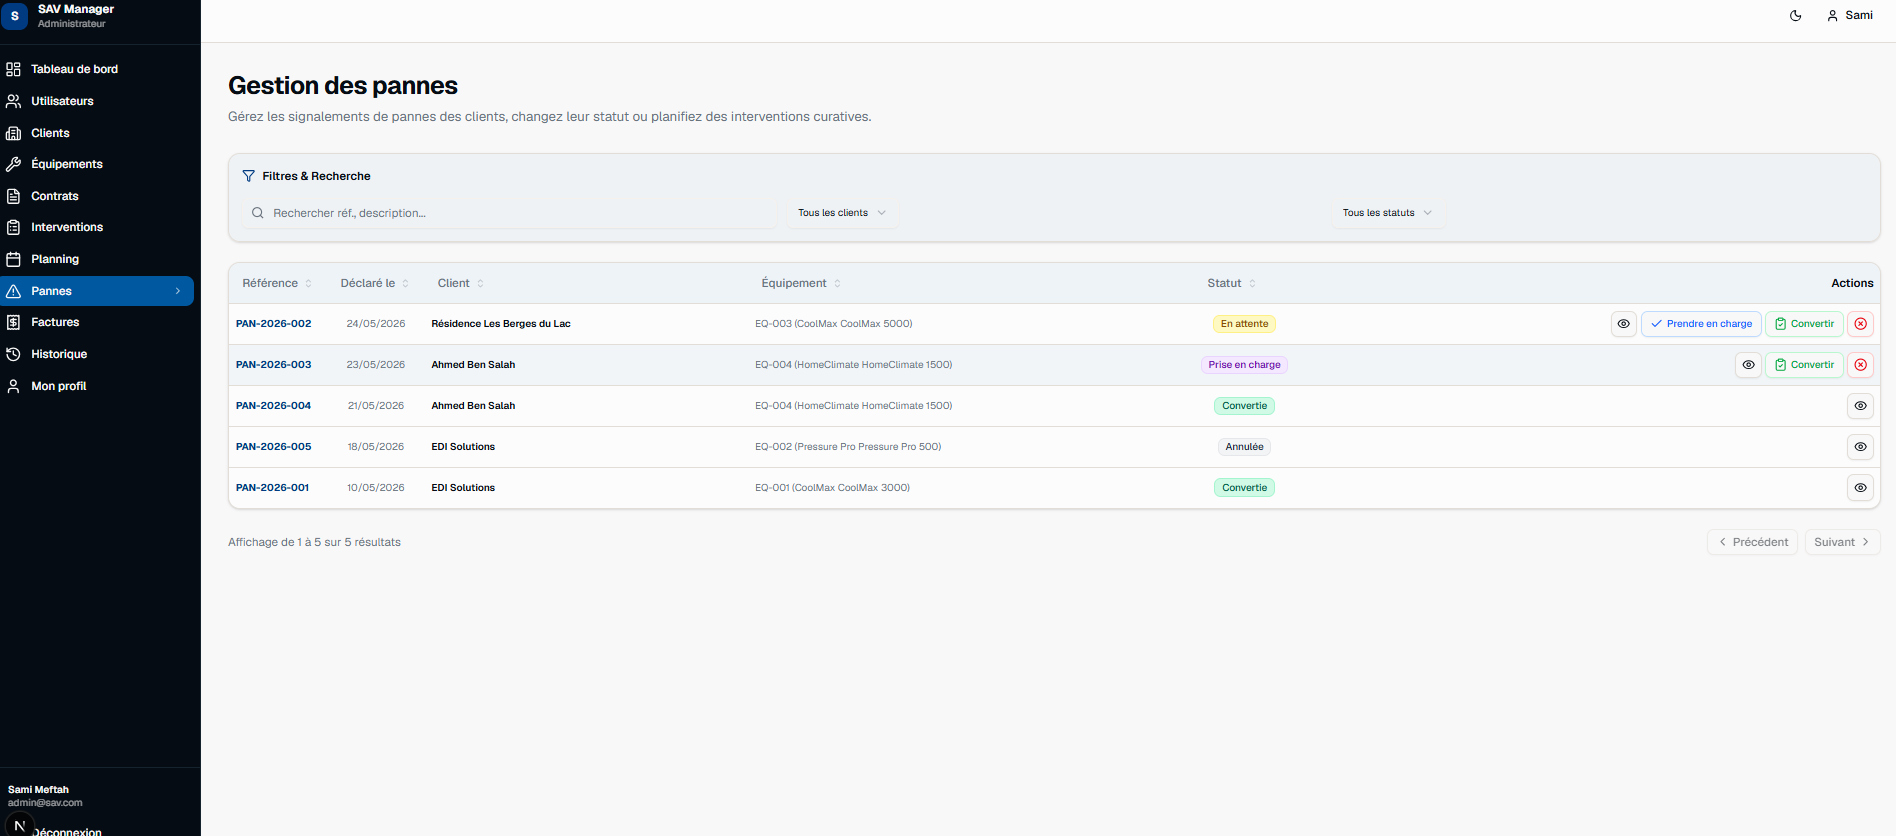
\includegraphics[width=0.74\textwidth]{Figures/Chapitre4/gestpannes.png}
    \caption{Capture d'écran : gestion des pannes}
    \label{fig:ch4:gestion_pannes}
\end{figure}

\begin{figure}[H]
\centering
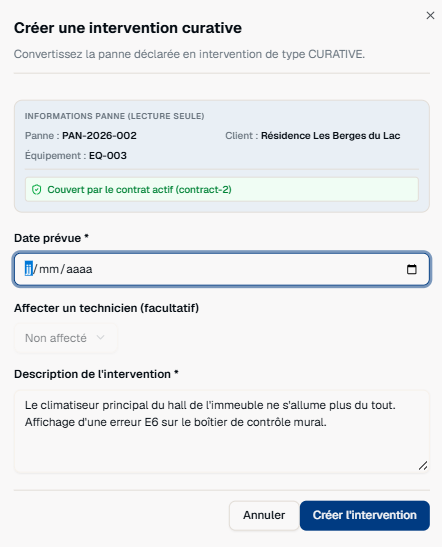
\includegraphics[width=0.45\textwidth]{Figures/Chapitre4/convertirpanne.png}
\caption{Capture d'écran : conversion d'une panne en intervention curative}
\label{fig:ch4:realisation_sprint2_pannes}
\end{figure}

% ─────────────────────────────────────────────────────────────────────────────
\section*{Conclusion}

Ce sprint a permis de développer le cœur fonctionnel du système SAV : la gestion complète du
cycle de vie des interventions préventives et curatives, la déclaration de pannes avec pièces
jointes par les clients, la conversion de pannes en interventions curatives, et la vérification
automatique de la couverture contractuelle. Le chapitre suivant présente le Sprint 3, dédié à la
facturation et aux tableaux de bord.
